\documentclass{standalone}
\usepackage{tikz}
\usetikzlibrary{patterns, positioning}


\begin{document}
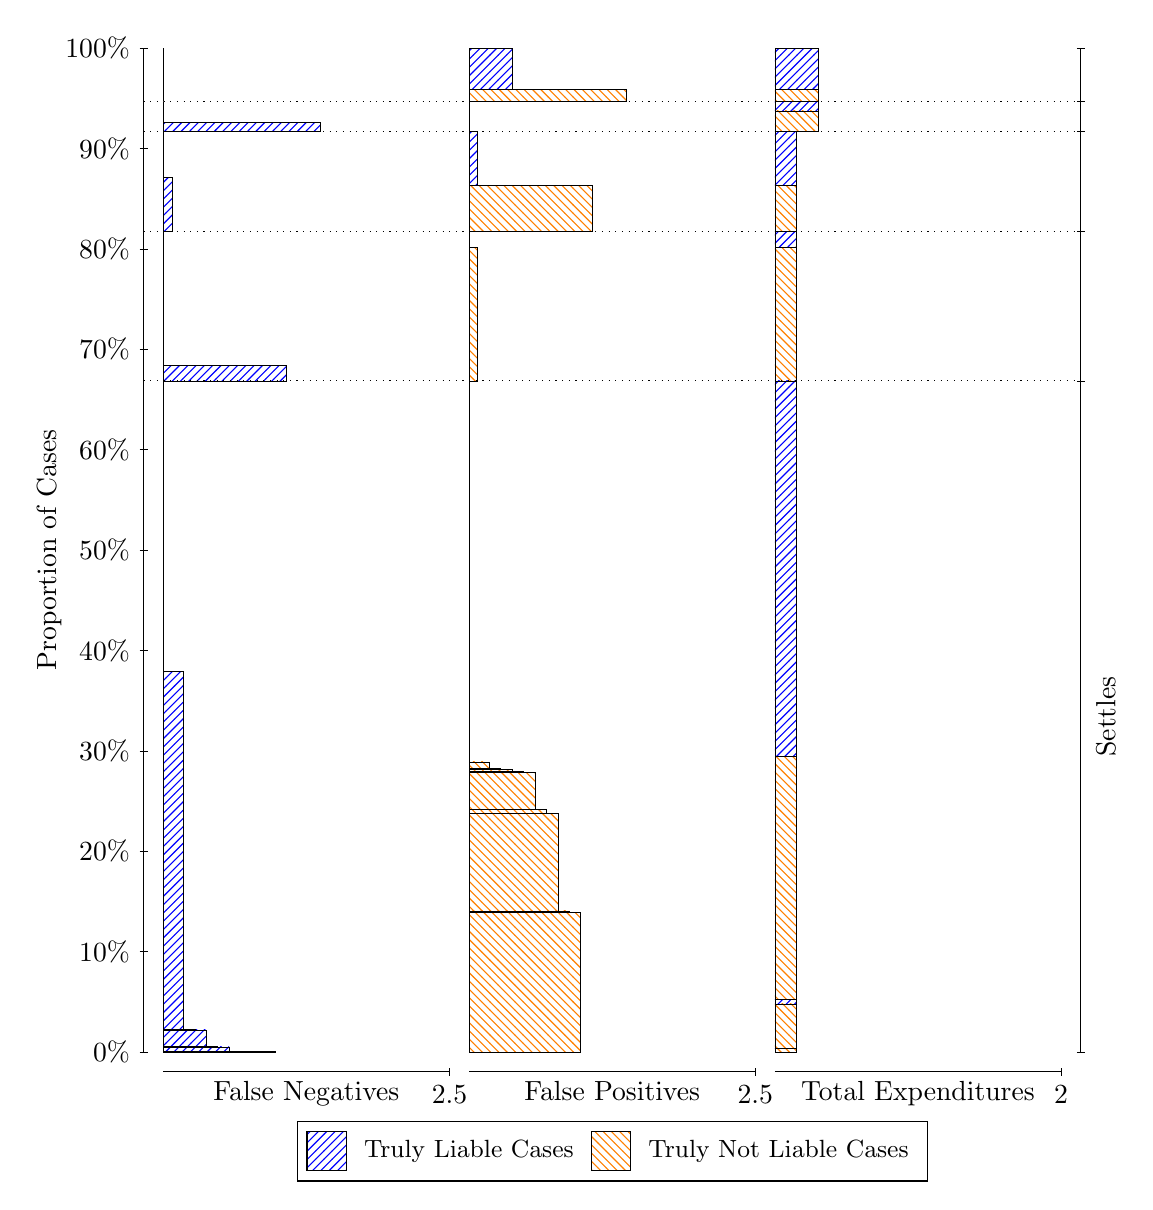
\begin{tikzpicture}
\draw[black, very thin] (1.5,1.75) -- (1.5,14.5);
\node[rotate=90, text=black, anchor=center] at (0.3, 8.125) {Proportion of Cases};
\draw[black, very thin] (1.45,1.75) -- (1.55,1.75);
\node[text=black, anchor=east] at (1.45, 1.75) {0\%};
\draw[black, very thin] (1.45,3.025) -- (1.55,3.025);
\node[text=black, anchor=east] at (1.45, 3.025) {10\%};
\draw[black, very thin] (1.45,4.3) -- (1.55,4.3);
\node[text=black, anchor=east] at (1.45, 4.3) {20\%};
\draw[black, very thin] (1.45,5.575) -- (1.55,5.575);
\node[text=black, anchor=east] at (1.45, 5.575) {30\%};
\draw[black, very thin] (1.45,6.85) -- (1.55,6.85);
\node[text=black, anchor=east] at (1.45, 6.85) {40\%};
\draw[black, very thin] (1.45,8.125) -- (1.55,8.125);
\node[text=black, anchor=east] at (1.45, 8.125) {50\%};
\draw[black, very thin] (1.45,9.4) -- (1.55,9.4);
\node[text=black, anchor=east] at (1.45, 9.4) {60\%};
\draw[black, very thin] (1.45,10.675) -- (1.55,10.675);
\node[text=black, anchor=east] at (1.45, 10.675) {70\%};
\draw[black, very thin] (1.45,11.95) -- (1.55,11.95);
\node[text=black, anchor=east] at (1.45, 11.95) {80\%};
\draw[black, very thin] (1.45,13.225) -- (1.55,13.225);
\node[text=black, anchor=east] at (1.45, 13.225) {90\%};
\draw[black, very thin] (1.45,14.5) -- (1.55,14.5);
\node[text=black, anchor=east] at (1.45, 14.5) {100\%};

\draw[black, very thin] (13.4,1.75) -- (13.4,14.5);
\draw[black, very thin] (13.35,1.75) -- (13.45,1.75);
\node[anchor=west] at (13.35, 1.75) {};
\draw[black, very thin] (13.35,10.272) -- (13.45,10.272);
\node[anchor=west] at (13.35, 10.272) {};
\draw[black, very thin] (13.35,12.171) -- (13.45,12.171);
\node[anchor=west] at (13.35, 12.171) {};
\draw[black, very thin] (13.35,13.439) -- (13.45,13.439);
\node[anchor=west] at (13.35, 13.439) {};
\draw[black, very thin] (13.35,13.82) -- (13.45,13.82);
\node[anchor=west] at (13.35, 13.82) {};
\draw[black, very thin] (13.35,14.5) -- (13.45,14.5);
\node[anchor=west] at (13.35, 14.5) {};

\draw[black, very thin, pattern color=blue, pattern=north east lines] (1.75,1.75) rectangle (3.167,1.755);
\draw[black, very thin, pattern color=blue, pattern=north east lines] (1.75,1.755) rectangle (3.0217,1.7555);
\draw[black, very thin, pattern color=blue, pattern=north east lines] (1.75,1.7555) rectangle (2.8763,1.7573);
\draw[black, very thin, pattern color=blue, pattern=north east lines] (1.75,1.7573) rectangle (2.731,1.7578);
\draw[black, very thin, pattern color=blue, pattern=north east lines] (1.75,1.7578) rectangle (2.5857,1.8147);
\draw[black, very thin, pattern color=blue, pattern=north east lines] (1.75,1.8147) rectangle (2.4403,1.8193);
\draw[black, very thin, pattern color=blue, pattern=north east lines] (1.75,1.8193) rectangle (2.295,2.0305);
\draw[black, very thin, pattern color=blue, pattern=north east lines] (1.75,2.0305) rectangle (2.1497,2.032);
\draw[black, very thin, pattern color=blue, pattern=north east lines] (1.75,2.032) rectangle (2.0043,6.5878);
\draw[black, very thin, pattern color=orange, pattern=north west lines] (1.75,6.5878) rectangle (1.75,10.272);
\draw[black, very thin, pattern color=blue, pattern=north east lines] (1.75,10.272) rectangle (3.3123,10.474);
\draw[black, very thin, pattern color=orange, pattern=north west lines] (1.75,10.474) rectangle (1.75,12.171);
\draw[black, very thin, pattern color=blue, pattern=north east lines] (1.75,12.171) rectangle (1.859,12.858);
\draw[black, very thin, pattern color=orange, pattern=north west lines] (1.75,12.858) rectangle (1.75,13.439);
\draw[black, very thin, pattern color=blue, pattern=north east lines] (1.75,13.439) rectangle (3.7483,13.558);
\draw[black, very thin, pattern color=orange, pattern=north west lines] (1.75,13.558) rectangle (1.75,13.82);
\draw[black, very thin, pattern color=orange, pattern=north west lines] (1.75,13.82) rectangle (1.75,13.97);
\draw[black, very thin, pattern color=blue, pattern=north east lines] (1.75,13.97) rectangle (1.75,14.5);
\draw[black, very thin, pattern color=orange, pattern=north west lines] (5.6333,1.75) rectangle (7.0503,3.5198);
\draw[black, very thin, pattern color=orange, pattern=north west lines] (5.6333,3.5198) rectangle (6.905,3.5411);
\draw[black, very thin, pattern color=orange, pattern=north west lines] (5.6333,3.5411) rectangle (6.7597,4.7833);
\draw[black, very thin, pattern color=orange, pattern=north west lines] (5.6333,4.7833) rectangle (6.6143,4.8274);
\draw[black, very thin, pattern color=orange, pattern=north west lines] (5.6333,4.8274) rectangle (6.469,5.3005);
\draw[black, very thin, pattern color=orange, pattern=north west lines] (5.6333,5.3005) rectangle (6.3237,5.3071);
\draw[black, very thin, pattern color=orange, pattern=north west lines] (5.6333,5.3071) rectangle (6.3237,5.309);
\draw[black, very thin, pattern color=orange, pattern=north west lines] (5.6333,5.309) rectangle (6.1783,5.3401);
\draw[black, very thin, pattern color=orange, pattern=north west lines] (5.6333,5.3401) rectangle (6.033,5.3475);
\draw[black, very thin, pattern color=orange, pattern=north west lines] (5.6333,5.3475) rectangle (5.8877,5.4346);
\draw[black, very thin, pattern color=blue, pattern=north east lines] (5.6333,5.4346) rectangle (5.6333,10.272);
\draw[black, very thin, pattern color=orange, pattern=north west lines] (5.6333,10.272) rectangle (5.7423,11.969);
\draw[black, very thin, pattern color=blue, pattern=north east lines] (5.6333,11.969) rectangle (5.6333,12.171);
\draw[black, very thin, pattern color=orange, pattern=north west lines] (5.6333,12.171) rectangle (7.1957,12.753);
\draw[black, very thin, pattern color=blue, pattern=north east lines] (5.6333,12.753) rectangle (5.7423,13.439);
\draw[black, very thin, pattern color=orange, pattern=north west lines] (5.6333,13.439) rectangle (5.6333,13.701);
\draw[black, very thin, pattern color=blue, pattern=north east lines] (5.6333,13.701) rectangle (5.6333,13.82);
\draw[black, very thin, pattern color=orange, pattern=north west lines] (5.6333,13.82) rectangle (7.6317,13.97);
\draw[black, very thin, pattern color=blue, pattern=north east lines] (5.6333,13.97) rectangle (6.1783,14.5);
\draw[black, very thin, pattern color=orange, pattern=north west lines] (9.5167,1.75) rectangle (9.7892,1.7971);
\draw[black, very thin, pattern color=blue, pattern=north east lines] (9.5167,1.7971) rectangle (9.7892,1.7999);
\draw[black, very thin, pattern color=orange, pattern=north west lines] (9.5167,1.7999) rectangle (9.7892,2.36);
\draw[black, very thin, pattern color=blue, pattern=north east lines] (9.5167,2.36) rectangle (9.7892,2.4219);
\draw[black, very thin, pattern color=orange, pattern=north west lines] (9.5167,2.4219) rectangle (9.7892,5.4993);
\draw[black, very thin, pattern color=blue, pattern=north east lines] (9.5167,5.4993) rectangle (9.7892,10.272);
\draw[black, very thin, pattern color=orange, pattern=north west lines] (9.5167,10.272) rectangle (9.7892,11.969);
\draw[black, very thin, pattern color=blue, pattern=north east lines] (9.5167,11.969) rectangle (9.7892,12.171);
\draw[black, very thin, pattern color=orange, pattern=north west lines] (9.5167,12.171) rectangle (9.7892,12.753);
\draw[black, very thin, pattern color=blue, pattern=north east lines] (9.5167,12.753) rectangle (9.7892,13.439);
\draw[black, very thin, pattern color=orange, pattern=north west lines] (9.5167,13.439) rectangle (10.062,13.701);
\draw[black, very thin, pattern color=blue, pattern=north east lines] (9.5167,13.701) rectangle (10.062,13.82);
\draw[black, very thin, pattern color=orange, pattern=north west lines] (9.5167,13.82) rectangle (10.062,13.97);
\draw[black, very thin, pattern color=blue, pattern=north east lines] (9.5167,13.97) rectangle (10.062,14.5);
\draw[black, dotted] (1.5,10.272) -- (13.4,10.272);
\draw[black, dotted] (1.5,12.171) -- (13.4,12.171);
\draw[black, dotted] (1.5,13.439) -- (13.4,13.439);
\draw[black, dotted] (1.5,13.82) -- (13.4,13.82);
\draw[black, very thin] (1.75,1.5) -- (5.3833,1.5);
\node[text=black, anchor=north] at (3.5667, 1.5) {False Negatives};
\draw[black, very thin] (5.3833,1.45) -- (5.3833,1.55);
\node[text=black, anchor=north] at (5.3833, 1.45) {2.5};

\draw[black, very thin] (5.6333,1.5) -- (9.2667,1.5);
\node[text=black, anchor=north] at (7.45, 1.5) {False Positives};
\draw[black, very thin] (9.2667,1.45) -- (9.2667,1.55);
\node[text=black, anchor=north] at (9.2667, 1.45) {2.5};

\draw[black, very thin] (9.5167,1.5) -- (13.15,1.5);
\node[text=black, anchor=north] at (11.333, 1.5) {Total Expenditures};
\draw[black, very thin] (13.15,1.45) -- (13.15,1.55);
\node[text=black, anchor=north] at (13.15, 1.45) {2};

\node[text=black, centered, rotate=90] at (13.72, 6.0112) {Settles};





\draw (7.449999999999999,1.5) node[draw=none] (baseCoordinate) {};
\begin{scope}[align=center]
        \matrix[scale=0.5, draw=black, below=0.5cm of baseCoordinate, nodes={draw}, column sep=0.1cm]{
            \node[rectangle, draw, minimum width=0.5cm, minimum height=0.5cm, pattern color=blue, pattern=north east lines] {}; &
            \node[draw=none, font=\small, text=black] (B) {Truly Liable Cases}; &
            \node[rectangle, draw, minimum width=0.5cm, minimum height=0.5cm, pattern color=orange, pattern=north west lines] {}; &
            \node[draw=none, font=\small, text=black] (B) {Truly Not Liable Cases}; \\
            };
\end{scope}

\end{tikzpicture}
\end{document}